\documentclass[11pt]{article}
\usepackage{graphicx}
\usepackage{caption}
\usepackage{subcaption}
%\usepackage{grffile}
%\usepackage{longtable}
%\usepackage{wrapfig}
%\usepackage{rotating}
%\usepackage[normalem]{ulem}
\usepackage{amsmath}
\usepackage{textcomp}
\usepackage{amssymb}
%\usepackage{capt-of}
\usepackage{hyperref}
\hypersetup{
    colorlinks=true,
    linkcolor=black,
    filecolor=blue,      
    urlcolor=blue,
    }
\usepackage{csquotes}
%\usepackage{fontspec} -- was added by org-mode
%\usepackage{newfloat}
%\usepackage{minted} -- was added by org-mode
\usepackage{booktabs}
\newcommand{\gr}[1]{\mathfrak{#1}}
\newcommand{\GG}{\gr{G}}
\newcommand{\VV}{\mathbb{V}}
\newcommand{\R}{\mathbb{R}}
\newcommand{\void}{\varnothing}
\newcommand{\unit}{\bullet}
\newcommand{\one}{\mathbf{1}}
\newcommand{\two}{\mathbf{2}}
\newcommand{\three}{\mathbf{3}}
\newcommand{\cell}{\mathbf{S}_\bullet}
\DeclareMathOperator{\reduce}{reduce}
\DeclareMathOperator{\map}{map}
\DeclareMathOperator{\zipWith}{zipWith}
\DeclareMathOperator{\fold}{fold}
\DeclareMathOperator{\scan}{scan}
\usepackage{xcolor}
\newcommand{\greycol}{black!20}
\newcommand{\grey}[1]{\textcolor{\greycol}{#1}}
\newcommand{\green}[1]{\textcolor{black!50!green}{#1}}
\author{Callum Mole}
\date{\today}
\title{Notes on Layout}
\begin{document}

\maketitle

\section{Introduction}

In `Grid types', James proposes an index type, \textit{Grid}, for building array-based generalised spreadsheets. We want to construct rules that converts the generalised spreadsheet to a data structure that can be represented in a familiar two dimensional spreadsheet layout, plus formatting. We will call this data structure a  `Spreadsheet', denoted $\mathbf{S}$. $\mathbf{S}$  should have within it all the layout and formatting information that the backends need to produce spreadsheets. The problem is a little circular: $\mathbf{S}$ should be able to extract the layout from the index types, but in order to type \textit{Grid} it would be helpful to know how the layout we wish to aim for. These notes are partly to help with my understanding of the problem, but hopefully also to help feed back into developing \textit{Grid}.


\section{\emph{Why} do we need types}

Statically typed languages can see into the future. They know what computations makes sense before they are executed. We need similar functionality to create spreadsheets. When faced with any given expression we should know how to represent its underlying structure, not simply evaluate the result. A typed language means that we are able to recover the structure of expressions, and hopefully represent this structure in the layout and formatting of the outputted spreadsheet. Furthermore, we can also be assured that we will not encounter expressions that have a structure we do not know about, so that our layout rules, once finalised, will be applicable to any expression they will encounter.


\section{Grid - recap}

A \emph{grid}, \(\gr{G}\), is a totally ordered, finite set. An \emph{array} is a map $\gr{G} \to P$, where  \(P\) is a set of all \emph{primitives}. We write \(\void\) for the empty grid (which is unique) and $\unit$ for a distinguished grid with a single element. 

A direct sum of grids, \(\bigoplus_i \GG_i\), is a an array of the length of all \(\GG\) combined but the output array knows how it got there. Conceptually, every grid is a direct sum of the unit grid $\unit$. For example, an array of type $\three \to P$ is a direct sum of three $\unit \to P$. Out of convenience we write an array of type $\unit\to P$ as a `bare value,' such as \verb|42|.

The direct product of grids is the Cartesian product with `dictionary order' on
the elements. We write the direct product of two grids, \(\gr{G}\) and
\(\gr{H}\), as \(\gr{G}\otimes\gr{H}\). The array \verb|[[10 20] [30 40] [50 60]]| is of type $\three \to (\two \to P)$, which is equivalent to $\three \bigotimes \two$. 

\section{Spreadsheet notation}

We keep in mind the difference between dimensions that have order, such as spatial layout and colour, and dimensions that are categorical, such as textual emphasis. We also note that as much as possible our formatting conventions should be generalisable to any output. Therefore, some dimensions that are not generalised to any output, for example colour, should be optional enhancements rather than a core way to communicate information.

For conciseness we will use the following notation to refer to spreadsheet representation. The final spreadsheet that is laid out and formatting we call $\mathbf{S}$. A double arrow $\Rightarrow$ represents the process of layout and formatting that produces $\mathbf{S}$. Everything to the left of $\Rightarrow$ is in the Cell domain, everything to the right of $\Rightarrow$ is in the $\mathbf{S}$ domain. The amount of cells covered is represented by a subscript 2D vector, such that 3 rows and 2 columns would be represented $\mathbf{S}_{[3,2]}$. For convenience a single cell is $\cell$   Spatial Layout is denoted by arrows ($\downarrow \rightarrow$). Colour is given by $\kappa$. If there is an order that is signified from less emphasis to more emphasis (e.g. light to dark) by $\overrightarrow{\kappa}$. Textual emphasis are indicated as follows: \textit{t}, \textbf{t}, \underline{t}. Borders, from dashed to solid to emphasised solid (could be double lines or bold): $\nmid, \mid, \parallel$. 

\section{Direct sums and spreadsheets} 

In $\mathbf{S}$ we should be able to distinguish between \verb|[10 20 30]| and \verb|{10 [20 30]}|. The first is $\one \bigoplus \one \bigoplus \one$ and the second is $\one \bigoplus \two$. 

An application is a sum type. For example the expression \verb|{+ 10 [20 30]}| has type $\one \bigoplus \one \bigoplus \two \to P$. Note that the expression \verb|{[+ +] [10 10] [20 30]}| has a different type of $\two \bigoplus \two \bigoplus \two \to P$. We may wish to represent these differently. 

Not all sum types are equal. The expression \verb|{10 10 [20 30]}|,  of type $\one \bigoplus \one \bigoplus \two$ may want to be treated differently than \verb|{+ 10 [20 30]}|, which is also of type $\one \bigoplus \one \bigoplus \two$.

For now we do not know how we want to represent applications. We first tackle the question:


\textit{How do we represent the structure of direct sums of grids when the primitives are bare values?}. 

Rule \ref{eq:rule1} states that all unit grids corresponds to a single spreadsheet cell. This seems uncontroversial for situations where the primitives are not applications.

\begin{equation} 
\unit \to P \Rightarrow \cell \label{eq:rule1}
\end{equation}

Next we need a rule to represent nested sums. Our array-based sum types can be represented as a hierachical tree structure (see `Grid Types'), where each grid of type $\unit \to P$ is a terminal node (or leaf). Note that at each level of the hierarchy there is also a \textit{horizontal} order, given by the grid index , meaning that our expressions are a sort of \href{https://en.wikipedia.org/wiki/Tree_(data_structure)#Ordered_tree}{ordered tree}. Fig \ref{fig:tree_examples} gives examples of various sum types that need to be principally converted into $\mathbf{S}$.

\subsection{A tree searching algorithm}

\begin{figure}[h] 
\centering
	\begin{subfigure}[b]{.3\textwidth}
		\centering
		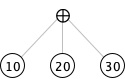
\includegraphics[scale=.5]{diags/tree1.png}
		\caption{{\texttt{[10 20 30]}}}\label{fig:a}
	\end{subfigure}	
	%%%%%%
  	\begin{subfigure}[b]{.3\textwidth}
  		\centering
    		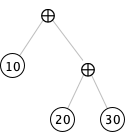
\includegraphics[scale=.5]{diags/tree2.png}
    		\caption{\texttt{\{[10 [20 30]\}}}\label{fig:b}
    \end{subfigure}
    %%%%%%
    \begin{subfigure}[b]{.3\textwidth}
    		\centering
    		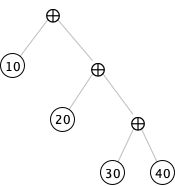
\includegraphics[scale=.5]{diags/tree3.png}
    		\caption{\texttt{\{10 \{20 [30 40]\}\}}}\label{fig:c}
    \end{subfigure}
    %%%%%
    \begin{subfigure}[b]{.45\textwidth}
    		\centering
    		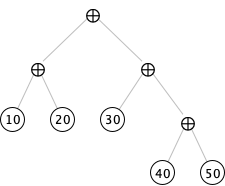
\includegraphics[scale=.5]{diags/tree4.png}
    		\caption{\texttt{\{[10 20] \{30 [40 50]\}\}}}\label{fig:d}
    \end{subfigure}
    %%%%%%
    \begin{subfigure}[b]{.45\textwidth}
    		\centering
    		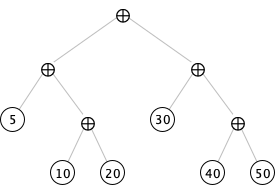
\includegraphics[scale=.5]{diags/tree5.png}
    		\caption{\texttt{\{\{5 [10 20]\} \{30 [40 50]\}\}}}\label{fig:e}
    \end{subfigure}
%%%%
    \begin{subfigure}[b]{.7\textwidth}
    		\centering
    		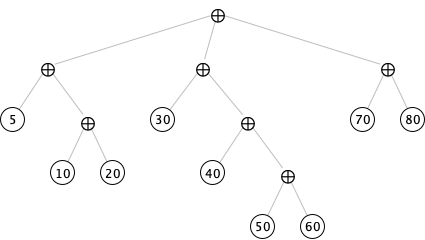
\includegraphics[scale=.5]{diags/tree6.png}
    		\caption{\texttt{\{\{5 [10 20]\} \{30 \{40 [50 60]\}\} [70 80]\}}}\label{fig:f}
    \end{subfigure}
  \caption{Examples of different Grid sum type structures}
  \label{fig:tree_examples}
\end{figure}

Before describing the formatting choices we make explicit our the expression tree is traversed. First, we start at the root node. At any point if the current node is the root node then the algorithm terminates. If the root node has child nodes, we count the length of the longest branch of each child, then order the children by the length, with longest branch first. We move to the first child, then map down to the first leaf of the longest branch.  In Fig \ref{fig:a} this would be \texttt{10}, in Fig \ref{fig:e} this would be \texttt{50}. At a leaf node (\textit{terminal node}) there are are two potential maps, to the next sibling node ($\overrightarrow{s}$), or to the parent node ($\uparrow_p$). Let $\overrightarrow{s}$ be the default map, with $\uparrow_p$ being executed only if there are no more sibling (child) nodes. 

If the current node is a parent node then it may have one or more sibling nodes, and we may have entered the set of sibling nodes at any position. Note that in our grid type system parent nodes are either direct sums or products (we will leave products for now), so in Fig \ref{fig:a} the parent node is \texttt{[10 20 30]}. If the parent node does not have siblings, it will be the root node, so the search will terminate. If current node has siblings, we map to the first sibling, ($\overleftarrow{s_1}$), which can be self-referential. If the new node has already been encountered, we map to the next sibling. If this sibling has child nodes we move to the deepest and leftmost leaf, $\swarrow_l$, and resume the left-right traverse as before.
\newline
\newline
\textit{Pseudocode notation}:
\begin{itemize}
	\item root, parent, leaf, child and sibling nodes as $r, p, l, c, s$ respectively
	\item current node is $\alpha$
	\item previously encountered nodes are in the list $\mathbf{e}$. 
	\item The set of parent nodes is $\mathbf{p}$.
	\item Position in the horizontal ordering is given by subscript $i$, e.g. $s_i$
	\item map direction is given by arrows.
	\item The shorthand $\swarrow_l$ means to recursively map to the child node with the longest branch until there are no more children, then map to the first sibling (i.e. the deepest, leftmost leaf). 
	\item $val$ refers to recording the node's value
\end{itemize}

\textit{Algorithm}: 

\begin{enumerate}
	\item Start at $r$.
	\item If $r \in \mathbf{p}$, then $\mathbf{c} = [c_i, c_{i+1} \dotsc c_n], \text{ where } depth(c_i) > depth(c_{i+1})$
	\item for $c$ in $\mathbf{c}:$
	\begin{enumerate}
			\item if $c \in \mathbf{p}$:
			\begin{enumerate}
				\item $\text{ do until } \alpha = c:$
				\begin{enumerate}
					\item if $\alpha \in \mathbf{p}: \:\swarrow_l$
					\item $val$
					\item  $\text{ do } \overrightarrow{s},val \text{ until } !\exists\; s_{i+1}$
					\item $\uparrow_p$.
					\item $\overleftarrow{s_1}, \text{do } \overrightarrow{s} \text{ until } \alpha \not\in \mathbf{e}$
					\item repeat for $s_i$s
				\end{enumerate}
				\item continue
			\end{enumerate}
			\item else, $val$, continue
	\end{enumerate}
\end{enumerate}

\subsection{Formatting the search}

It should be clear from the formatting how the tree has been traversed. In the following description the algorithm steps are translated to formatting steps. Algorithm steps that do not need to be represented in the formatted are coloured \grey{grey}. Formatting steps are coloured \green{green} for ease of reading.

\begin{enumerate}
	\item Start at $r$ \green{$\Rightarrow $ new column (enter heading...)}
	\item \grey{If $r \in \mathbf{p}$, then $\mathbf{c} = [c_i, c_{i+1} \dotsc c_n], \text{ where } depth(c_i) > depth(c_{i+1})$}
	\item \grey{for $c$ in $\mathbf{c}:$}
	\begin{enumerate}
			\item if $c \in \mathbf{p}$: \green{$\Rightarrow$ if it isn't the first child add an empty row}
			\begin{enumerate}
				\item \grey{$\text{ do until } \alpha = c:$}
				\begin{enumerate}
					\item if $\alpha \in \mathbf{p}: \:\swarrow_l$  \green{$\Rightarrow$ add a dashed border}
					\item $val$  \green{$\Rightarrow$ enter value in current cell}
					\item  $\text{ do } \overrightarrow{s},val \text{ until } !\exists\; s_{i+1}$ \green{$\Rightarrow$ for each sibling, move down a cell and enter value}
					\item $\uparrow_p$. \green{$\Rightarrow$ add a solid border}
					\item \grey{$\overleftarrow{s_1}, \text{do } \overrightarrow{s} \text{ until } \alpha \not\in \mathbf{e}$}
					\item \grey{repeat for $s_i$}
				\end{enumerate}
				\item \grey{continue}
			\end{enumerate}
			\item else, $val$, continue \green{$\Rightarrow$ enter value into current cell, move down a cell}
	\end{enumerate}
\end{enumerate}


In other words, the formatting rules, where $x$ is a node and only leaf nodes return $value(x)$, are:


\begin{align}
\bigoplus_i \gr{G}_i &\Rightarrow \text{a column} \\
value(x) &\Rightarrow \text{cell value}\\ 
deepestleaf(x) &\Rightarrow \text{dashed border}\\
sibling(x) &\Rightarrow \text{no border} \\
parent(x) &\Rightarrow \text{solid border}\\
branch?(x) &\Rightarrow \text{empty row if not the first and has more than 1 level}
\end{align} \label{eq:rule2}

These rules would give the following formatting for the examples in Fig \ref{fig:tree_examples}.

\begin{figure}[h] 
\centering
	\begin{subfigure}[b]{.3\textwidth}
		\centering
		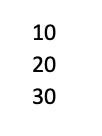
\includegraphics[scale=.5]{screenshots/format1.png}
		\caption{{\texttt{[10 20 30]}}}\label{fig:fa}
	\end{subfigure}	
	%%%%%%
  	\begin{subfigure}[b]{.3\textwidth}
  		\centering
    		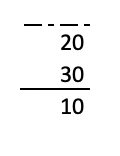
\includegraphics[scale=.5]{screenshots/format2.png}
    		\caption{\texttt{\{[10 [20 30]\}}}\label{fig:fb}
    \end{subfigure}
    %%%%%%
    \begin{subfigure}[b]{.3\textwidth}
    		\centering
    		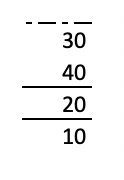
\includegraphics[scale=.5]{screenshots/format3.png}
    		\caption{\texttt{\{10 \{20 [30 40]\}\}}}\label{fig:fc}
    \end{subfigure}
    %%%%%
    \begin{subfigure}[b]{.45\textwidth}
    		\centering
    		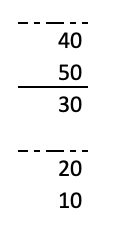
\includegraphics[scale=.5]{screenshots/format4.png}
    		\caption{\texttt{\{[10 20] \{30 [40 50]\}\}}}\label{fig:fd}
    \end{subfigure}
    %%%%%%
    \begin{subfigure}[b]{.45\textwidth}
    		\centering
    		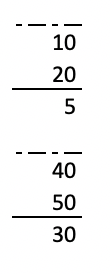
\includegraphics[scale=.5]{screenshots/format5.png}
    		\caption{\texttt{\{\{5 [10 20]\} \{30 [40 50]\}\}}}\label{fig:fe}
    \end{subfigure}
%%%%
    \begin{subfigure}[b]{.7\textwidth}
    		\centering
    		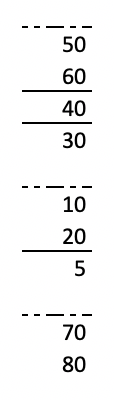
\includegraphics[scale=.5]{screenshots/format6.png}
    		\caption{\texttt{\{\{5 [10 20]\} \{30 \{40 [50 60]\}\} [70 80]\}}}\label{fig:ff}
    \end{subfigure}
  \caption{Examples of formatting for the Grid sum type structures shown in Fig \ref{fig:tree_examples}}
  \label{fig:format_examples}
\end{figure}









\end{document}
